% Compression rewrite (DECISION-20261119c; REWRITE-RULES-20261119.md rule 5): text the cov2d lane moved verbatim out of
% the posted note's Part 5, with one move-manifest row per sentence (CV-P5 ids in
% history-cuts/move-manifest-cv-part5-20261119.tsv). References into the note resolve through main_note.aux (xr).
\section{Validation detail moved from the note}
This section holds supporting detail that the compressed note's Part 5 no longer prints, as the note printed it.

\subsection{Closure detail (from Part 5, closures)}
% From sec_q3_closure.tex:9 (draft lineage of 5d7210adc)
Both residuals are at least $30\times$ below the threshold: OmniFold recovers the injected truth shape.

% From sec_q3_3d.tex:5 (draft lineage of 5d7210adc)
Total normalization matches to better than \SI{1}{\percent}.

% From sec_q3_3d.tex:5 (draft lineage of 5d7210adc)
In the metric of \S\ref{sec:validation} ($\Eavail$ projection) the residual is \SI{1.84}{\percent} against \SI{18.1}{\percent} injected (ratio $0.102$).

% From sec_q3_3d.tex:8 (draft lineage of 5d7210adc)
The closure's marginal scatter is far below the $\SI{3.7}{\percent}$ data-versus-2D scatter.

% From sec_q3_3d.tex:8 (draft lineage of 5d7210adc)
The data comparison sets configuration (e) against configuration (f), a cross-configuration comparison.

% From sec_q3_3d.tex:8 (draft lineage of 5d7210adc)
That comparison's scatter is therefore not interpreted as data--simulation structure resolved by the available-energy axis, and the ratio of the two scatters is not quoted.

% From sec_q3_3d.tex:8 (draft lineage of 5d7210adc)
The hidden-variable closure exceeds its threshold at the largest amplitude (\S\ref{sec:validation}, App.~\ref{app:response-mismatch}).

\subsection{Five-dimensional estimator development detail (from Part 5, P5-3)}
% The director's ruling of 2026-11-19 (P5-3 item 3): development history on the baseline and probe classifiers and
% the procedure detail behind Part 5's findings, moved verbatim (rows CV-P5-3.* in
% history-cuts/move-manifest-cv-part5-20261119.tsv).

% From sec_5d.tex:88 (draft 6ed12eed4)
The binned unfolding unfolds the same simulated events [as the boosted-tree comparison of the note's \S\ref{sec:val-departure}], with their exact efficiency and the response binned in the 10,499 occupied five-dimensional reconstructed cells, starting from the nominal prior.

% From sec_5d.tex:90 (draft 6ed12eed4)
Of the 144 eligible residuals, pooled over the deformations, 15 are dominated by the tree approximation. Only 2 of these 15 lie in identified quantities, a share of 0.014 of the 144. An identified quantity has a relative Cram\'er--Rao width at or below \SI{2.5}{\percent} at the analysis exposure. A width between that bound and the \SI{10}{\percent} bound is neither. Of the 144, 121 lie in quantities that the binned response constrains weakly at the analysis exposure. Their Cram\'er--Rao widths exceed \SI{10}{\percent} at both truth resolutions tested (median \SI{31}{\percent} at the coarser resolution, that of the J cells themselves). Here the regularization trades a large variance for the bias.

% From sec_5d.tex:92 (draft 6ed12eed4)
Longer noise-free exact iteration removes much of the residual for D1 (J median \SI{3.3}{\percent} after 200 iterations and \SI{0.8}{\percent} after $10^{5}$) and part of it for W1 (\SI{3.3}{\percent} and \SI{2.8}{\percent}). It does not do so for W3 and the $q_3$ stress (\SI{4.4}{\percent} and \SI{6.6}{\percent} after 200 iterations, \SI{8.9}{\percent} and \SI{6.7}{\percent} after $10^{5}$), whose within-cell binning bias grows with the iteration number. The long runs do not converge (only 9--34 of the 109 J quantities converge for each traced deformation). These values are last iterates. The coarser muon projection retained only three cases and is uninformative.

% From sec_5d.tex:129 (draft 6ed12eed4)
The scalar five-dimensional estimator studied here uses production LightGBM.

% From sec_5d.tex:133 (draft 6ed12eed4)
The noise-free study unfolds the full simulation's reweighted reconstructed events without background. Baseline classifiers and the missed-event regressor use 100 trees and 8 leaves; the capacity probe uses 400 trees and 31 leaves.

% From sec_5d.tex:139 (draft 6ed12eed4)
Saved fine-grid outputs are integrated into the supported J, H2 and EW cells of the table below [the label table of the note's \S\ref{sec:gbdt-model-dependence}]. Unsupported cells remain in the full-domain rate. The interval assessment keeps all 42 EW cells, including the three that the support rule excludes (definitions and normalization checks in App.~\ref{sec:gbdt-diagnostic-definitions}).

% From sec_5d.tex:159 (draft 6ed12eed4)
\paragraph{Recovery changes, but not uniformly.}

% From sec_5d.tex:161 (draft 6ed12eed4)
Figure~\ref{fig:gbdt-recovery} shows the traces over the recorded iteration ranges (later checkpoint entries are excluded, App.~\ref{sec:gbdt-diagnostic-definitions}); none is extrapolated. D1 and W1 improve slowly. W3's J-cell median absolute residual rises from \SI{5.57}{\percent} at iteration 5 to \SI{6.57}{\percent} at 200, and its maximum from \SI{32.9}{\percent} to \SI{44.8}{\percent}. The corresponding H2 medians are \SI{3.42}{\percent} and \SI{3.68}{\percent}. The persistence of the W3 residual is established over this finite scan only, not for unlimited iterations or for every possible classifier. The $q_3$ stress shows how much the functional matters: its EW median residual rises from \SI{4.99}{\percent} at iteration 5 to \SI{6.42}{\percent} at 30 even while some joint-cell summaries improve.

% From sec_5d.tex:163 (draft 6ed12eed4)
The capacity probe changes recovery. Its recorded traces reach 10 iterations (Fig.~\ref{fig:gbdt-recovery}); five iterations is the most the computing budget allowed at that capacity, and that is the comparison used here. At that point the larger classifiers lower the largest residual proxy over the development truths (lower row of Fig.~\ref{fig:gbdt-recovery}) by 3\% on J and 8\% on H2, short of the improvement of at least 20\% required before the larger capacity would be used.

% From sec_5d.tex:165 (draft 6ed12eed4)
Because the measure [the largest residual proxy over the development truth changes, the note's \S\ref{sec:gbdt-model-dependence}] is a maximum over the truth changes, the slow gains for D1 and W1 do not lower the measure: on H2, over the noise-free traces of Fig.~\ref{fig:gbdt-recovery}, it is 0.314 at five iterations and at least 0.384 at 10, 15 or 20.

% From sec_5d.tex:189-196 (draft 6ed12eed4)
\begin{figure}[tbp]
\centering
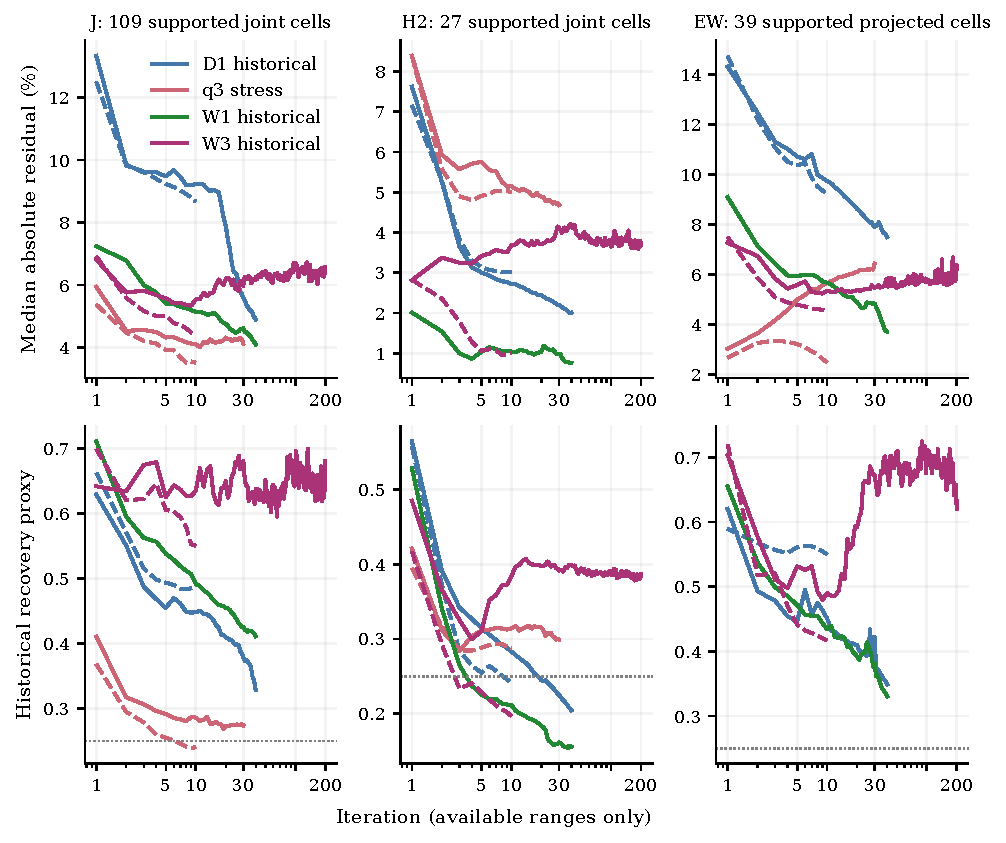
\includegraphics[width=\linewidth]{figures/gbdt_recovery.pdf}

\caption[Noise-free five-dimensional recovery against iterations]{In noise-free development traces, more iterations reduce the D1 and W1 residuals only slowly, and the W3 residual persists over the scan. Historical truth ratios, fixed simulated detector response. Solid/dashed OmniFold curves: 100 trees/8 leaves and 400/31. Iteration maxima: D1/W1 40, $q_3$ 30, W3 200, capacity probes 10. Some baseline traces end at their last saved checkpoint. Top: median $|\hat f/f_{\rm true}-1|$ over supported cells. Bottom: residual proxy $\operatorname{median}(|\hat f/f_{\rm true}-1|/|f_{\rm true}/f_0-1|)$ for departures above 1\%, dotted bound 0.25. Different denominators prevent reading one minus this proxy as an exact recovered fraction. The $q_3$ stress has no eligible EW departure. These traces measure no repeat variance.}

\label{fig:gbdt-recovery}
\end{figure}

% From sec_5d.tex:211 (draft 6ed12eed4)
At nominal truth, EW41 contains the truth in 15 of 40 68\% intervals (37.5\%, pointwise exact 95\% interval [22.7\%, 54.2\%]), so a pooled pass cannot qualify this cell. A check with the width averaged over several bootstrap estimates is in App.~\ref{app:devhistory}.

% From sec_5d.tex:225 (draft 6ed12eed4)
Twenty edge-safe data jitters (uniform input perturbations within half a single-precision unit in the last place that keep the fine-grid membership fixed) give a J-cell median SD of \SI{0.228}{\percent}, against a bootstrap SD of \SI{0.368}{\percent}.

% From sec_q3_fived16.tex:118 (draft 6ed12eed4)
At the two flagged truths, the root-mean-square bias of IBU at five iterations over the sixteen cells and its noise-free $\chi^2$ are \fvval{prr-cmp-gibuu} than configuration~(e)'s at the GiBUU hybrid truth and \fvval{prr-cmp-q3} at the $q_3$ tilt (Table~\ref{tab:fived16-prr}).

% From sec_q3_fived16.tex:120-134 (draft 6ed12eed4)
\begin{table}[htbp]
\centering\small
\caption[Retained prior at the two flagged truths]{At both flagged truths, IBU at five iterations overshoots the truth along the prior-to-truth direction, while configuration~(e) retains part of each departure. Retained fraction $\rho$, root-mean-square over the sixteen cells of the bias $b_c$, which is relative to the prior cross section, and noise-free $\chi^2$ (16 degrees of freedom) at the two flagged truths, for configuration~(e) and IBU at five iterations, on noise-free pseudo-data at one simulation split. A negative $\rho$ means that, along the prior-to-truth direction, the result overshoots the truth; the total bias is in the RMS and $\chi^2$ columns.}
\label{tab:fived16-prr}
\begin{tabular}{lcccccc}
\toprule
 & \multicolumn{2}{c}{$\rho$} & \multicolumn{2}{c}{RMS bias} & \multicolumn{2}{c}{$\chi^2$} \\
\cmidrule(lr){2-3}\cmidrule(lr){4-5}\cmidrule(lr){6-7}
truth & (e) & IBU & (e) & IBU & (e) & IBU \\
\midrule
GiBUU hybrid & $\fvval{prr-rho-e-gibuu}$ & $\fvval{prr-rho-ibu-gibuu}$ & \fvval{prr-rms-e-gibuu} & \fvval{prr-rms-ibu-gibuu} & \fvval{prr-chi2-e-gibuu} & \fvval{prr-chi2-ibu-gibuu} \\
$q_3$ tilt & $\fvval{prr-rho-e-q3}$ & $\fvval{prr-rho-ibu-q3}$ & \fvval{prr-rms-e-q3} & \fvval{prr-rms-ibu-q3} & \fvval{prr-chi2-e-q3} & \fvval{prr-chi2-ibu-q3} \\
\bottomrule
\end{tabular}
\end{table}

% From sec_q3_fived16.tex:138 (draft 6ed12eed4)
Reducing the iteration count from \fvval{prr-s53-b0-iters} to \fvval{prr-s53-k2-iters} increased $\rho$ beyond the threshold at the $q_3$ tilt. These settings [the reduced iteration count above, and the reduced capacity and $(\pT,\pPar)$-only learners of the note's \S\ref{sec:fived16-prr}] also newly flagged \fvval{prr-lev-K2-nnew}, \fvval{prr-lev-C25-nnew} and \fvval{prr-lev-O2-nnew} of the other \fvval{prr-lev-nother-word} graded truths, respectively, in the noise-free study. For \fvval{prr-pr1-noeffect}, no change as large as the threshold is detected. Every higher iteration count and capacity tested lowers $\rho$ at both truths, by at most \fvval{prr-more-dmax}, less than the threshold.

\subsection{Fake-data and unfolding-algorithm detail (from Part 5, P5-4a)}
% The director's approved P5-4 plan (2026-11-19): procedure and descriptive detail behind Part 5's fake-data and IBU
% findings, moved verbatim (rows CV-P5-4a.* in history-cuts/move-manifest-cv-part5-20261119.tsv).

% From sec_q3_fived16.tex:36 (draft 190331a95)
The methods paper withholds this second rule's counts [V-PRIOR, the note's \S\ref{sec:fived16-fd}], because its generator spread uses the CH-corrected NuWro and GiBUU predictions (\S\ref{sec:joint5d-ch}). The counts remain the recorded classification.

% From sec_q3_fived16.tex:44 (draft 190331a95)
A descriptive comparison made after the grades, against smaller matrices, finds the biases, apart from the listed truths, small next to the reported covariance and, apart from the two closures at the prior, large next to its statistical block alone. It changes no grade.

% From sec_q3_fived16.tex:47 (draft 190331a95)
The other eight control checks [besides the failed offset check, the note's \S\ref{sec:fived16-fd}] passed.

% From sec_q3_fived16.tex:49-72 (draft 190331a95)
\begin{table}[htbp]
\centering\footnotesize
\caption[Descriptive fake-data numbers]{Descriptive fake-data numbers only, without test outcomes. In-sample: reported $C_{\mathrm{total}}+C_{\mathrm{resp}}+C_{\mathrm{PL,5D}}$, including the truth's generator shift, supplies no evidence (--- where the test already uses the full matrix). Model-only: statistical block plus $C_{\mathrm{model}}$ without that shift, omitting interaction, flux, detector, lateral and normalization blocks, gives a lower bound on $C_{\mathrm{model}}$'s reach. Power alternatives on Tune~v1 (r) and GENIE CV (g): NuWro $(\pT,\pPar,\Eavail)$ shape (P1), NuWro $q_3$ shape at fixed $(\Eavail,W)$ (P2), GENIE + MEC $(\Eavail,W)$ shape (P3).}
\label{tab:fived16-fdvar}
\scriptsize\setlength{\tabcolsep}{3pt}
\begin{tabular}{@{}lrrr@{\qquad}lrrr@{}}
\toprule
truth & \multicolumn{2}{c}{in-sample $\chi^2$, $p$} & model-only $\chi^2$ & power alternative & $n$ & $\chi^2$ & $p$ \\
\midrule
simulation prior (MINERvA Tune~v1) & --- & --- & \fvval{f0b-nominal-model_only-chi2} & P1r & \fvval{f0b-P1r-n} & \fvval{f0b-P1r-chi2} & $\fvval{f0b-P1r-p}$ \\
MINERvA Tune~v1, hybrid & --- & --- & \fvval{f0b-A7_mnvtune-model_only-chi2} & P2r & \fvval{f0b-P2r-n} & \fvval{f0b-P2r-chi2} & $\fvval{f0b-P2r-p}$ \\
GENIE CV, hybrid & --- & --- & \fvval{f0b-A7_genie_cv-model_only-chi2} & P3r & \fvval{f0b-P3r-n} & \fvval{f0b-P3r-chi2} & $\fvval{f0b-P3r-p}$ \\
GENIE + MEC, hybrid & \fvval{f0b-A7_genie_mec-in_sample-chi2} & $\fvval{f0b-A7_genie_mec-in_sample-p}$ & \fvval{f0b-A7_genie_mec-model_only-chi2} & P1g & \fvval{f0b-P1g-n} & \fvval{f0b-P1g-chi2} & $\fvval{f0b-P1g-p}$ \\
GENIE + MEC, $(\Eavail,W)$ shape (W2) & \fvval{f0b-W2-in_sample-chi2} & $\fvval{f0b-W2-in_sample-p}$ & \fvval{f0b-W2-model_only-chi2} & P2g & \fvval{f0b-P2g-n} & \fvval{f0b-P2g-chi2} & $\fvval{f0b-P2g-p}$ \\
NuWro, hybrid & \fvval{f0b-A7_nuwro-in_sample-chi2} & $\fvval{f0b-A7_nuwro-in_sample-p}$ & \fvval{f0b-A7_nuwro-model_only-chi2} & P3g & \fvval{f0b-P3g-n} & \fvval{f0b-P3g-chi2} & $\fvval{f0b-P3g-p}$ \\
NuWro, $\Eavail$ shape (W1) & \fvval{f0b-W1-in_sample-chi2} & $\fvval{f0b-W1-in_sample-p}$ & \fvval{f0b-W1-model_only-chi2} & & & & \\
NuWro, $(\pT,\pPar,\Eavail)$ shape (W3) & \fvval{f0b-W3-in_sample-chi2} & $\fvval{f0b-W3-in_sample-p}$ & \fvval{f0b-W3-model_only-chi2} & & & & \\
NuWro, closure (noise-free) & \fvval{f0b-closure_nuwro-in_sample-chi2} & $\fvval{f0b-closure_nuwro-in_sample-p}$ & \fvval{f0b-closure_nuwro-model_only-chi2} & & & & \\
GiBUU, $\Eavail$ shape & \fvval{f0b-stage0c_gibuu-in_sample-chi2} & $\fvval{f0b-stage0c_gibuu-in_sample-p}$ & \fvval{f0b-stage0c_gibuu-model_only-chi2} & & & & \\
GiBUU, hybrid & \fvval{f0b-A7_gibuu-in_sample-chi2} & $\fvval{f0b-A7_gibuu-in_sample-p}$ & \fvval{f0b-A7_gibuu-model_only-chi2} & & & & \\
synthetic $q_3$ tilt & --- & --- & \fvval{f0b-q3-model_only-chi2} & & & & \\
\bottomrule
\end{tabular}
\end{table}

% From sec_q3_fived16.tex:75 (draft 190331a95)
Each tune enters as its normalized shape ratio to GENIE CV on the fine grid, constructed as the reweighting ratios of the $C_{\mathrm{model}}$ shifts are. Where the tune's sample fails the ratio's statistical gate, the ratio is pooled over a coarser cell or set to one. The ratio is applied to the simulated truth, under the simulation's detector response.

% From sec_q3_fived16.tex:77 (draft 190331a95)
The mean of the pseudo-experiments gives $\chi^2=\fvval{f1-g18-chi2}$ ($p=\fvval{f1-g18-p}$; largest $|z|$ \fvval{f1-g18-zmax}, in \fvval{f1-g18-zcell}) at \fvval{f1-tune-g18} and \fvval{f1-ar23-chi2} ($p=\fvval{f1-ar23-p}$; \fvval{f1-ar23-zmax}, in \fvval{f1-ar23-zcell}) at \fvval{f1-tune-ar23}; the closures give \fvval{f1-closure-g18-chi2} ($p=\fvval{f1-closure-g18-p}$; \fvval{f1-closure-g18-zmax}, in \fvval{f1-closure-g18-zcell}) and \fvval{f1-closure-ar23-chi2} ($p=\fvval{f1-closure-ar23-p}$; \fvval{f1-closure-ar23-zmax}, in \fvval{f1-closure-ar23-zcell}). This group has \fvval{f1-grp-zcells} of \fvval{f1-grp-cells} cells with $|z|>\fvval{trig-z}$ (Gaussian reference \fvval{f1-grp-refcells}) and \fvval{f1-grp-ptruths} of \fvval{f1-grp-truths} records with $p<\fvval{trig-p}$ (reference \fvval{f1-grp-reftruths}). The four records are the pseudo-experiment and closure results for two truths, so the Gaussian references, which count them as independent, are context only.

% From sec_q3_fived16.tex:79 (draft 190331a95)
The two tunes use the same quasielastic cross-section model, GENIE's \texttt{NievesQELCCPXSec}, \fvval{f1-tune-ar23} with a z-expansion form factor, and the MEC model of \fvval{f1-tune-g18} is of the Valencia family used in the GENIE + MEC shift. Descriptively, without the GENIE + MEC shift, the pseudo-experiments give $\chi^2=\fvval{f1-g18-sens-chi2}$ ($p=\fvval{f1-g18-sens-p}$) and \fvval{f1-ar23-sens-chi2} ($p=\fvval{f1-ar23-sens-p}$), and the closures \fvval{f1-closure-g18-sens-chi2} ($p=\fvval{f1-closure-g18-sens-p}$) and \fvval{f1-closure-ar23-sens-chi2} ($p=\fvval{f1-closure-ar23-sens-p}$). The model-only $\chi^2$, defined as in Table~\ref{tab:fived16-fdvar}, are \fvval{f1-mo-chi2-min}--\fvval{f1-mo-chi2-max} in the four records, with cell \fvval{f1-ar23-mo-cells} beyond $\fvval{trig-z}\sigma$ at \fvval{f1-tune-ar23} in both its records. Rerunning the tests with the two tunes added reproduces every earlier fake-data result exactly.

% From sec_q3_fived16.tex:128 (draft 190331a95)
Descriptively, at a NuWro closure the IBU's median absolute residual is \lrval{rg1-r2-nuwro} times that of configuration~(e), and at the simulation's own truth, a trivial closure, the IBU's residual vanishes; neither is a coverage statement for either estimator.

\subsection{Five-dimensional estimator tests in full (from Part 5, P5-Q1)}
% DECISION-20261120a and the director's approved P5-Q plan (2026-11-20): the sentences of the note's sec_5d.tex that
% the condensed note no longer prints, moved verbatim and in order (rows CV-P5-Q1.* in
% history-cuts/move-manifest-cv-part5-20261119.tsv). The note's pointer: "supporting detail of these studies is in the records document".

\paragraph{From the note's \S\ref{sec:5d}.}
% From sec_5d.tex:5 (draft de1543818)
[The note's \S\ref{sec:5d}:] It covers what each test isolates (\S\ref{sec:val-fiveaxis}), background subtraction and generator-sized truth changes (\S\ref{sec:val-negweight}), why the estimator does not follow such changes (\S\ref{sec:val-departure}), model dependence and the reporting definitions it rules out (\S\ref{sec:gbdt-model-dependence}), the coverage test (\S\ref{sec:coverage-5d}) and the status of the five-axis covariance of the \resFiveAxis{} (\S\ref{sec:eavailw-construction}; configurations in Table~\ref{tab:config-key}). The sixteen-cell result of the \estMultiD{} is given in \S\ref{sec:fived16}, and the calibrated generator tests built on a variant of this estimator in \S\ref{sec:joint5d}. The unbinned negative-weight background method itself is derived in App.~\ref{app:negweight}.

\paragraph{From the note's \S\ref{sec:val-fiveaxis}.}
% From sec_5d.tex:9 (draft de1543818)
Prior reweighting changes the frequencies of existing simulated truth events while retaining their detector-response simulation. A response mismatch instead changes how a given truth is reconstructed. Finite classifier capacity and iteration count approximate the inverse and can leave residuals in either case. Coverage asks whether the resulting intervals contain their specified target at the stated rate (\S\ref{sec:coverage-5d}). These mechanisms are separate: an incorrect generator prediction alone does not diagnose an interval failure. Each test below [in the note, \S\S\ref{sec:val-negweight}--\ref{sec:eavailw-construction}] isolates one intervention.

\paragraph{From the note's \S\ref{sec:val-negweight}.}
% From sec_5d.tex:24 (draft de1543818)
Without background, the same experiments [the note's end-to-end five-dimensional pseudo-experiments at nominal truth, here run without background events] recover the truth to \SI{0.22}{\percent}.
% From sec_5d.tex:34 (draft de1543818)
The \SI{74}{\percent} residual is in the cell $0.8\le\Eavail<\SI{1.5}{GeV}$, $W\ge\SI{3}{GeV}$, whose share of the cross section the deformation study did not record.
% From sec_5d.tex:43 (draft de1543818)
[For the \estMultiD{}'s recovered-fraction grade at the GiBUU-to-GENIE change and the three withheld shapes:] Its residual is the mean over 20 pseudo-experiments with backgrounds at each of these truths, each against its own half-sample truth. [At the GiBUU-to-GENIE change:] Of the \fvval{rec-g-n} supported cells with an injected change of magnitude above \SI{\fvval{rec-thr}}{\percent}, \fvval{rec-g-opp} move opposite to it and \fvval{rec-g-over} overshoot it. In the cell $0.8\le\Eavail<\SI{1.5}{GeV}$, $W\ge\SI{3}{GeV}$, the injected change is $\fvval{rec-g-ew29-inj}\,\%$, but the unfolded value lies \SI{\fvval{rec-g-ew29-unf}}{\percent} above the nominal truth.

\paragraph{From the note's \S\ref{sec:val-departure}.}
% From sec_5d.tex:51 (draft de1543818)
With noise-free pseudo-data the unfolding recovers more than \SI{99}{\percent} of the change that the departure produces in the reconstructed distribution, whereas the median $(\Eavail,W)$ truth residual ranges from \SI{5}{\percent} to \SI{11}{\percent}, with \SI{74}{\percent} in the worst cell. The unrecovered reconstructed-level difference is small relative to the departure but statistically significant at the analysis exposure.
% From sec_5d.tex:53 (draft de1543818)
A larger classifier improves the reconstructed-level fit without reducing the $\Eavail$ truth residual, and removing the regression for events that fail reconstruction does not reduce that residual either.
% From sec_5d.tex:60 (draft de1543818)
[In the comparison with exact binned unfolding:] At five iterations the J-cell medians of the absolute residual agree: \SI{9.5}{\percent}, \SI{5.4}{\percent}, \SI{5.6}{\percent} and \SI{4.3}{\percent} for the boosted trees, against \SI{8.3}{\percent}, \SI{5.4}{\percent}, \SI{4.9}{\percent} and \SI{5.3}{\percent} for the exact binned unfolding, for D1, W1, W3 and the $q_3$ stress.
% From sec_5d.tex:71 (draft de1543818)
The instability [the \estMultiD{}'s data-stability failure under rounding-level input changes] also explains the difference of at most \SI{1.2}{\percent} on data between the driver and the development pipeline.
% From sec_5d.tex:78 (draft de1543818)
[The ensemble-averaged variant of the \estMultiD{} fails its no-worse closure requirement only at the GiBUU $\Eavail$ shape.] There, on noise-free fake data, its root-mean-square closure bias is \fvval{ens1-g-rms-r} against \fvval{ens1-g-rmsc-r} for the \estMultiD{}, about \fvval{ens1-g-rms-dpct}\,\% larger. The excess is \fvval{ens1-g-drms} against a noise floor of \fvval{ens1-g-floor}, or \fvval{ens1-g-ratio} times the floor. In noise-free fake-data closures at the other \fvval{ens1-nnoworse} of the \fvval{ens1-ntruths} distinct truths, it is no worse than the \estMultiD{}. On the sixteen cells of the data (\S\ref{sec:fived16}), the ensemble average differs from the reported result by at most \SI{\fvval{e96d-maxpct}}{\percent}, and by at most \fvval{e96d-maxsig} of a cell's standard deviation from $C_{\mathrm{e}}$ (\S\ref{sec:fived16-cov}). Its fits perturb a float64 copy of the inputs at the rounding level. On the unperturbed copy, the \estMultiD{} gives the reported result to double precision.

\paragraph{From the note's \S\ref{sec:gbdt-model-dependence}.}
% From sec_5d.tex:99 (draft de1543818)
[Estimator $R$:] With seed 42, its 40 nominal experiments and 20 at each of five departures include Poisson pseudo-data, changing MC splits and background refinement.
% From sec_5d.tex:136 (draft de1543818)
The selection procedure then takes RD3 as the fallback, and RD3 fails the total-width target.
% From sec_5d.tex:149 (draft de1543818)
At historical W3 truth, EW29 has mean residual \SI{23.67}{\percent} and repeat SD \SI{0.56}{\percent}; EW7 has \SI{-6.81}{\percent} and \SI{0.30}{\percent}. Coarser cells can have smaller residuals and spread, but they estimate different integrals, so their smaller residuals and spread are not an improvement in precision on an unchanged quantity.
% From sec_5d.tex:155 (draft de1543818)
[Caption of the note's Fig.~\ref{fig:gbdt-bias-spread}, continued:] Each supported J or H2 cell gives the mean and SD of $(\hat f-f_{\rm true})/f_{\rm true}$ in the same background-inclusive ensemble: 40 nominal experiments, 20 each for W2 and W3. Bars give pointwise 95\% Student-$t$ intervals for means and normal-model intervals for SDs, conditional on saved simulation. They supply neither simultaneous bounds nor total uncertainties. Truth panels and reporting cells form no frontier across estimator settings.
% From sec_5d.tex:168 (draft de1543818)
[Caption of the note's Fig.~\ref{fig:gbdt-coverage}, continued:] Below: EW7 ($\Eavail\in[0.1,0.2)$, $W\in[1.1,1.4)$ GeV) and EW41 (both above 3 GeV), pointwise 95\% Clopper--Pearson bounds. Dotted: nominal Gaussian 68.27\%. Neither total uncertainty nor a newly validated interval is shown. The bootstrap $\sigma$ is from 100 replicas of the nominal seed 700000; the assessment samples are reused, and no per-experiment or total-coverage claim is made.
% From sec_5d.tex:184 (draft de1543818)
[Caption of the note's Fig.~\ref{fig:gbdt-prior}, continued:] Historical W3 at five iterations. Horizontal gives minus the noise-free relative truth residual; vertical gives the relative shift in real-data $R$ when its MC prior changes to W3, normalized to CV-prior results. Points are supported cells, not independent repeated experiments. The diagonal marks equality.

\paragraph{From the note's \S\ref{sec:coverage-5d}.}
% From sec_5d.tex:215 (draft de1543818)
[Caption of the note's Fig.~\ref{fig:coverage-5d-paper}, continued:] Circles/squares: 68\%/95\% intervals. Bars: one-sided Clopper--Pearson lower/upper bounds at level $0.05/459$ (Bonferroni: 153 integrals, three truths). Solid/dashed: nominal coverage/thresholds 0.66 and 0.94. Filled: upper bound below threshold. Nominal truth (undrawn): none below 0.66, two below 0.94. Order: 42 $(\Eavail,W)$ cells and sum, \jtNcells{} joint cells (indices in $3^5$), total.

\paragraph{From the note's \S\ref{sec:eavailw-construction}.}
% From sec_5d.tex:271 (draft de1543818)
A 160-throw ensemble determines a standard deviation only to a relative precision of about $1/\sqrt{2(N-1)}\approx\SI{5.6}{\percent}$ for independent Gaussian throws, so a smaller seed-induced drift could not be resolved against the width it would change.
% From sec_5d.tex:274 (draft de1543818)
[Item 2 of the note's list of what the covariance supports:] Within the limits stated below, the sensitivity is not the statistic's own resampling noise, which would fall with $N$. The same-seed resampling floor falls steeply from $\floorNforty\,\%$ at $N=40$ to $\floorNeighty\,\%$ at $N=80$, with two-point exponent $\floorExponent$; no floor measurement exists at $N=160$. Three limits rule out a statement about infinite ensembles. First, the $40$- and $80$-throw points are nested subsets of the same 160 throws, not independent ensembles. The flatness [of the seed sensitivity over the 40-, 80- and 160-throw ensembles, stated in the note] therefore holds within one ensemble, over a factor of four in $N$; the behavior at larger $N$ is unmeasured. Second, the scatter of these subset means, $\pm\seedEffectScatter\,\%$, is at a single seed pair (offsets $\{0,1200\}$); the width of the distribution over seed pairs is unmeasured. Third, the statistic is a maximum over the specified offset set, so additional pairs can only raise it.
% Search: floor at N=160; larger ensemble; seed-pair width; seed pairs (values.tex:446 "the FLOOR was measured at N=40 and N=80 ONLY"; nd-unfolding/CORRECTED_UQ_PRODUCTION_STATUS.md:17-22, the 40- and 80-throw points nested in one 160-throw ensemble at one seed pair; CORRECTION-20260921-seed-effect-larger-ensemble-corollary-withdrawn.md:71-74, the N=160 floor of EVIDENCE-20260920 is an extrapolation; release-package-20260922/README.md:35-39, larger N and the seed-pair width unmeasured) @ 624acea1 [carried from sec_5d.tex:275]
% From sec_5d.tex:276 (draft de1543818)
[Of the five bands that fall outside the seed variation (item 3):] Allowing them to vary could move the total in either direction, and neither is measured, because $s_{\mathrm{proj}}$ maximizes relative changes over functionals rather than summing nonnegative component contributions.
% From sec_5d.tex:277 (draft de1543818)
[Item 4:] Individual five-axis bins reach $\cvMoveBinOverSigmaMax\,\%$ of their uncertainty; summing bins suppresses this movement in projections.

\paragraph{From the note's Table~\ref{tab:test-index}.}
% From part5_validation.tex (draft de1543818)
[Injected $W$ bump (5D), Outcome cell, after ``pass, by a narrow margin'':] Neighboring $W$ bins \SI{3.1}{\percent} and \SI{2.7}{\percent} high; per-5D-bin spread \SI{3.7}{\percent}

\subsection{Fake-data, closure and classifier detail (from Part 5, P5-Q2)}
% DECISION-20261120a and the director's approved P5-Q plan (2026-11-20): sentences of the note's sec_q3_fived16.tex,
% sec_q3_bias.tex and sec_q3_3d.tex that the condensed note no longer prints, moved verbatim and in order (rows
% CV-P5-Q2.* in history-cuts/move-manifest-cv-part5-20261119.tsv). Bracketed words are context, not the note's.

\paragraph{From the note's \S\ref{sec:3d-closure}.}
% From sec_q3_bias.tex:21 (draft 16e2dfe7b)
[For the note's injected $\Eavail$ bump, unfolded with the \estPurity{}:] The recovered step-2 mean weight is $1.048$ against the injected $1.0485$. Residuals against reweighted truth on the $\Eavail$-marginal have median $0.9999$ and standard deviation \textbf{\num{0.0006}} (\SI{0.06}{\percent}).

\paragraph{From the note's \S\ref{sec:fived16-fd}.}
% From sec_q3_fived16.tex:33 (draft 16e2dfe7b)
[The listings of the note's fake-data tests use the reported construction of $C_{\mathrm{model}}$.] If $C_{\mathrm{model}}$ is built with GiBUU's ratio on the generators' common phase space, the listed truths are the same; this construction cannot change the grades of the two GiBUU truths, because their grading covariances omit GiBUU's component. If it is built from smoothed ratios, the NuWro hybrid truth is also listed, by its $p$ alone ($p=\fvval{rsn-sm-nuwro-p}$, no cell beyond $\fvval{trig-z}\sigma$). Under both constructions, the held-out tunes still meet both bias criteria.
% From sec_q3_fived16.tex:44 (draft 16e2dfe7b)
[Of the three groups of the note's fake-data truths, evaluated separately:] Under the reported covariance, the $C_{\mathrm{model}}$-generator truths have \fvval{f0b-grp-vertex-family-zcells} of \fvval{f0b-grp-vertex-family-cells} cells with $|z|>\fvval{trig-z}$ (Gaussian reference \fvval{f0b-grp-vertex-family-refcells}) and \fvval{f0b-grp-vertex-family-ptruths} of \fvval{f0b-grp-vertex-family-truths} truths with $p<\fvval{trig-p}$ (reference \fvval{f0b-grp-vertex-family-reftruths}); the other truths \fvval{f0b-grp-non-vertex-zcells} of \fvval{f0b-grp-non-vertex-cells} and \fvval{f0b-grp-non-vertex-ptruths} of \fvval{f0b-grp-non-vertex-truths}; and the prior truths \fvval{f0b-grp-prior-zcells} of \fvval{f0b-grp-prior-cells} and \fvval{f0b-grp-prior-ptruths} of \fvval{f0b-grp-prior-truths}. The Gaussian references are context only, because the bias is deterministic.

\paragraph{From the note's \S\ref{sec:fived16-ibu}.}
% From sec_q3_fived16.tex:100 (draft 16e2dfe7b)
[Between the note's sixteen cells and the binned IBU unfolding of the same data:] The largest differences, IBU minus the \estMultiD{} as fractions of the \estMultiD{}, are $\fvval{ibu16-dof-R11}\,\%$ in R11, $\fvval{ibu16-dof-R06}\,\%$ in R06 and $\fvval{ibu16-dof-R05}\,\%$ in R05, or \fvval{ibu16-dsig-R11}, \fvval{ibu16-dsig-R06} and \fvval{ibu16-dsig-R05} times each cell's reported standard deviation; over the sixteen cells the difference reaches \fvval{ibu16-dsig-max} times a cell's reported standard deviation.
% From sec_q3_fived16.tex:103 (draft 16e2dfe7b)
[In the same comparison:] The IBU uncertainty is a median \lrval{rg1-r3-med} times that of the \estMultiD{} over the sixteen cells (\lrval{rg1-r3-lo}--\lrval{rg1-r3-hi}); the \estMultiD{}'s statistical block includes its estimator's own noise, refit per replica, and the IBU has none.

\paragraph{From the note's \S\ref{sec:3d-classifier}.}
% From sec_q3_3d.tex:9 (draft 16e2dfe7b)
[Caption of the note's Fig.~\ref{fig:calibration}, continued:] The five-iteration OmniFold cross-check uses identical weighted 3D inputs and extraction, changing only the classifier family. The MLP/GBDT total-cross-section ratio is $1.0078$; median absolute projection differences are \SI{1.20}{\percent} in $\pT$, \SI{1.36}{\percent} in $\pPar$, and \SI{0.66}{\percent} in $\Eavail$.

\subsection{Caption detail (caption pass, Part 4)}
% The director's ruling of 2026-11-20 (option (a)): secondary caption sentences of Part 4, moved verbatim (rows
% CV-CAP4.* in history-cuts/move-manifest-cv-captions-20261120.tsv). Bracketed words are context, not the note's.

% From sec_fived16_gen.tex:112 (draft d55f7aad6)
[Caption of the note's Fig.~\ref{fig:fived16-modes}, continued:] Predictions use analysis definitions.

% From sec_fived16_gen.tex:177 (draft d55f7aad6)
[Caption of the note's Table~\ref{tab:fived16-gen-cmodel}, continued:] The CH column is this note's sensitivity, omitted by the methods paper because it uses the free-proton samples of \S\ref{sec:joint5d-ch}.

% From sec_3d.tex:93 (draft d55f7aad6)
[Caption of the note's Fig.~\ref{fig:eavail-marg}, continued:] See the \estPurity{} definition in the method configurations (\S\ref{sec:method-config}).

% From sec_3d.tex:132 (draft d55f7aad6)
[Caption of the note's Fig.~\ref{fig:3dmodels}, continued:] The fourth-axis comparison (\S\ref{sec:4d}) gives $\Eavail$-marginal data/Tune~v1 ratios.

% From sec_3d.tex:170 (draft d55f7aad6)
[Caption of the note's Fig.~\ref{fig:modedecomp}, continued:] The remainder of the gap [the low-$\Eavail$ data$-$CV gap left after GENIE regenerated with Valencia 2p2h closes about half of it, in central values] occupies the region the MINERvA tune's empirical enhancement is built to absorb.

% From sec_3d.tex:202 (draft d55f7aad6)
[Caption of the note's Fig.~\ref{fig:q3excess}, continued:] See the \estPurity{} method definition (\S\ref{sec:method-config}).

\subsection{Caption detail (caption pass, Parts 2, 3, 5 and appendices)}
% The director's ruling of 2026-11-20 (option (b)): secondary caption sentences outside Part 4, moved verbatim (rows
% CV-CAPR.* in history-cuts/move-manifest-cv-captions-20261120.tsv). Bracketed words are context, not the note's.

% From app_negweight.tex:87 (draft d55f7aad6)
[Caption of the note's Fig.~\ref{fig:negweight-ratio}, continued:] [the low-$p_T$, high-background edge bin of the negative-weight/purity ratio map] Background is largest in the edge bin, and the $\max(0,\cdot)$/structural floor of \S\ref{sec:negweight-estimator} governs the result there.

% From sec_experiment.tex:52 (draft d55f7aad6)
[Caption of the note's Fig.~\ref{fig:control-corner}, continued:] [among the simulation's pairwise correlations of the five reconstructed observables] The strongest correlations share recoil energy, $q_{3}$ with $\Eavail$ ($r\approx0.81$) and $W$ with $\Eavail$ ($r\approx0.73$), or the muon transverse kick, $q_{3}$ with $\pT$ ($r\approx0.59$).

% From sec_experiment.tex:52 (draft d55f7aad6)
[Caption of the note's Fig.~\ref{fig:control-corner}, continued:] Apart from $\Eavail$ with $\pT$ ($r\approx0.34$), $\Eavail$ and $W$ are nearly uncorrelated with the muon variables.

% From sec_joint.tex:85 (draft d55f7aad6)
[Caption of the note's Table~\ref{tab:joint5d}, continued:] [the six conditions under which every joint test is rejected] The conditions concern (i) the null truth below the fine grid, (ii) the detector model, (iii) the interaction-model prior, (iv) the simulation size, (v) the neutrino-energy range and (vi) the predictions' own finite simulated samples (\S\ref{sec:joint5d-conditions}).

% From sec_joint.tex:111 (draft d55f7aad6)
[Caption of the note's Fig.~\ref{fig:joint5d-nulls}, continued:] Sufficient inputs: App.~\ref{app:release}.

% From sec_results.tex:111 (draft d55f7aad6)
[Caption of the note's Fig.~\ref{fig:ptslices}, continued:] Only the panel format follows Fig.~13 of Ref.~\cite{MINERvA:2021owq}.

% From sec_results.tex:111 (draft d55f7aad6)
[Caption of the note's Fig.~\ref{fig:ptslices}, continued:] Published-data comparisons are in Figs.~\ref{fig:xsec} and~\ref{fig:pull} and Table~\ref{tab:compare}.

% From sec_results.tex:193 (draft d55f7aad6)
[Caption of the note's Fig.~\ref{fig:modelmaps}, continued:] [our result's and the published data's ratio maps to MINERvA Tune~v1] The maps are close because both results depart from the tune in the same places by similar amounts.

% From selection_features.tex:6 (draft d55f7aad6)
[Caption of the note's Table~\ref{tab:selection-features}, continued:] Extended fiducial domain: App.~\ref{sec:fps}.
